\documentclass{beamer}
\usepackage[italian]{babel}
\usepackage{multicol}

\usepackage{tikz}
\usepackage{graphicx}
\usepackage[table, x11names]{xcolor}
\usepackage{xstring}
\usepackage{etoolbox}
\usepackage{tabularx}
\usepackage[export]{adjustbox}
\usepackage[font=tiny]{caption}

\newcommand{\Date}{}

\newcommand{\setDate}[1]{\renewcommand{\Date}{#1}}

\useinnertheme{default}
\useoutertheme{default}
\usecolortheme{default}

\definecolor{aziendaPrimary}{RGB}{84, 150, 104}
\setbeamercolor{structure}{fg=aziendaPrimary}
\setbeamercolor{frametitle}{bg=aziendaPrimary!10,fg=aziendaPrimary}

% rimuovere i simboli di navigazione
\setbeamertemplate{navigation symbols}{}


% pagina iniziale
\setbeamertemplate{title page}{
  \vspace{4em}
  \begin{center}
    \hspace{1.5cm}
    \begin{minipage}{0.3\textwidth}
      \centering
      
\includegraphics[height=2.5cm, right]{../logo-crop.pdf}
    \end{minipage}
    \begin{minipage}{0.3\textwidth}
      \centering
      
\includegraphics[height=2.5cm, left]{img/logounipd.png}
    \end{minipage}
  \end{center}
  \begin{center}
    \vspace{0.5em}
      {\usebeamerfont{title}\color{black}\textbf{\inserttitle}\par}
    \vspace{0.7em}
    {\usebeamerfont{date}\insertauthor\par}
    \vspace{0.5cm}
    {\usebeamerfont{date}\Date\par}
  \end{center}
}

% footer
\setbeamertemplate{footline}{
  \vspace{2ex}
  \hbox{
    \begin{minipage}[t]{0.40\paperwidth}
      \hspace*{0.5em}
      \raggedright\usebeamerfont{footline}{Presentazione architettura 20/04/2026}
    \end{minipage}%
    \begin{minipage}[t]{0.20\paperwidth}
      \centering\usebeamerfont{footline}Slide \insertframenumber{} di \inserttotalframenumber
    \end{minipage}%
    \begin{minipage}[t]{0.40\paperwidth}
      \hfill
      \insertshortauthor
      \hspace*{0.8em}
      \raisebox{-0.25\height}{
\includegraphics[width=0.7cm]{../logo-crop.pdf}}
      \hspace*{1.3em}
    \end{minipage}
  }
  \vspace{0.8ex}
}

\usepackage[absolute,overlay]{textpos}

\title{Presentazione architettura}
\author[]{Gruppo 1 - A.A 2025/2026}
\setDate{20/04/2026}

\begin{document}
{
\setbeamertemplate{footline}{}
\begin{frame}
  \titlepage
\end{frame}
}

\begin{frame}{Obiettivo capitolato}
\begin{itemize}
  \item Capitolato C9 (Vimar View4Life): Piattaforma per la gestione degli impianti Smart nelle residenze protette;
  \item Sistema di gestione allarmi e utenti (OSS e Amministrazione) che possono interagire con gli allarmi (gestione e risoluzione);
  \item Visualizzazione di statistiche sui consumi, con relativi consigli per ridurli, e sugli allarmi.
\end{itemize}
\begin{center}
    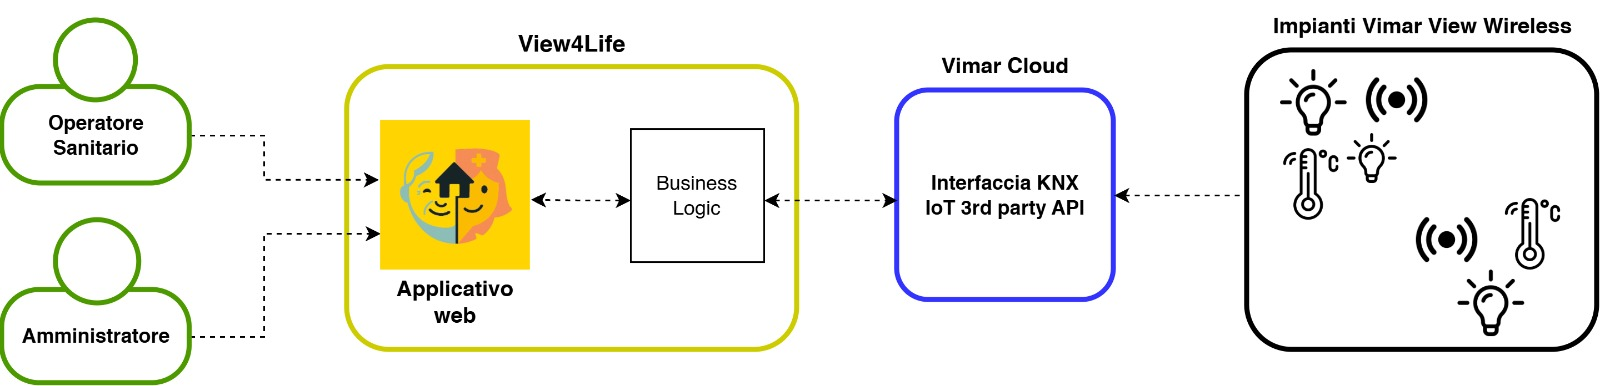
\includegraphics[width=0.75\textwidth]{img/schemacapitolato.jpeg}\\
\end{center}
\end{frame}

\begin{frame}{Architettura di deployment}
\begin{itemize}
  \item Frontend: \textit{Single Page Application} in Angular, servita da \textit{nginx};
  \item Backend: monolite realizzato con NestJS.
\end{itemize}
\vspace{0.2cm}
Entrambi, come il database \textit{PostgreSQL}, sono containerizzati e orchestrati da \textit{Docker Compose}. 
\vspace{0.2cm}

Attualmente tutti e tre i container sono in esecuzione in un singolo nodo.
\end{frame}

\begin{frame}{Backend: Architettura esagonale}
\begin{itemize}
  \item Problema:
  \begin{itemize}
    \item La logica di business del \textit{backend} dipende dai dettagli infrastrutturali (\textit{Persistent Logic});
    \item Difficile testare il \textit{backend} senza dover istanziare l'intera infrastruttura.
  \end{itemize}
  \item Soluzione: \textbf{Architettura Esagonale}
        \begin{itemize}
          \item Il dominio non dipende da componenti esterne;
          \item Le \textbf{Ports} sono interfacce \textit{TypeScript} che il dominio espone, 
                gli \textbf{Adapters} le implementano;
          \item Le dipendenze tra i moduli sono risolte tramite il \textit{pattern} \textbf{Dependency Injection}.
        \end{itemize}
\end{itemize}
\end{frame}

\begin{frame}{UML Alarm (Backend) (1/2)}
\begin{center}
   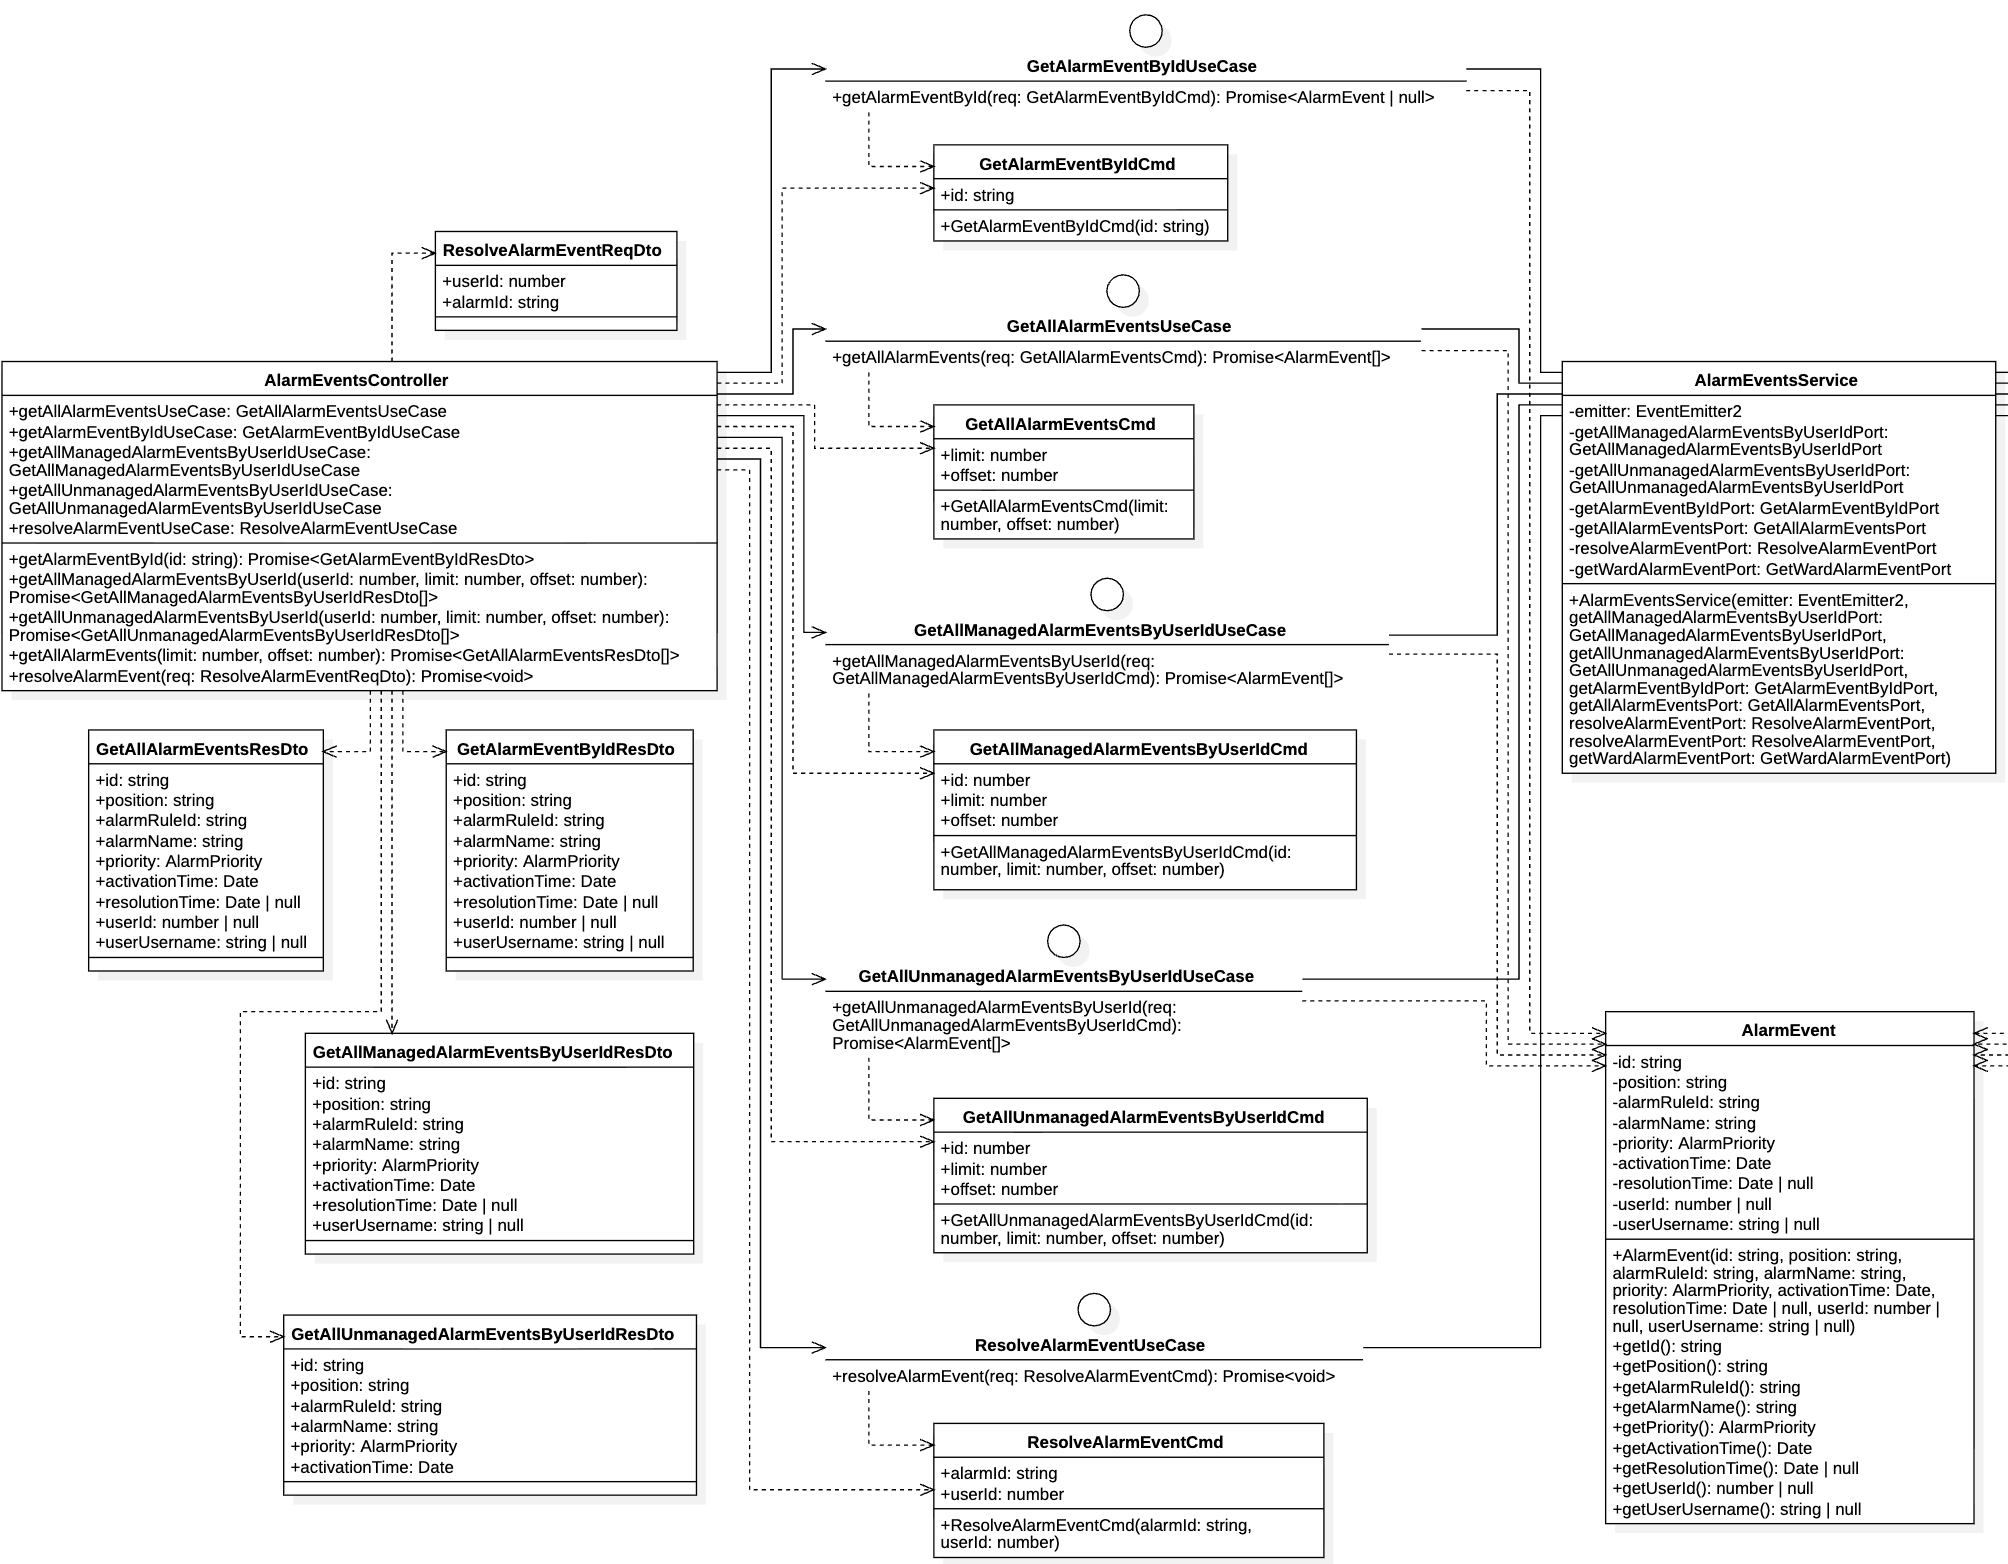
\includegraphics[width=0.95\textwidth]{img/AlarmUML.png}
\end{center}
\end{frame}

\begin{frame}{UML Alarm (Backend) (2/2)}
\begin{center}
   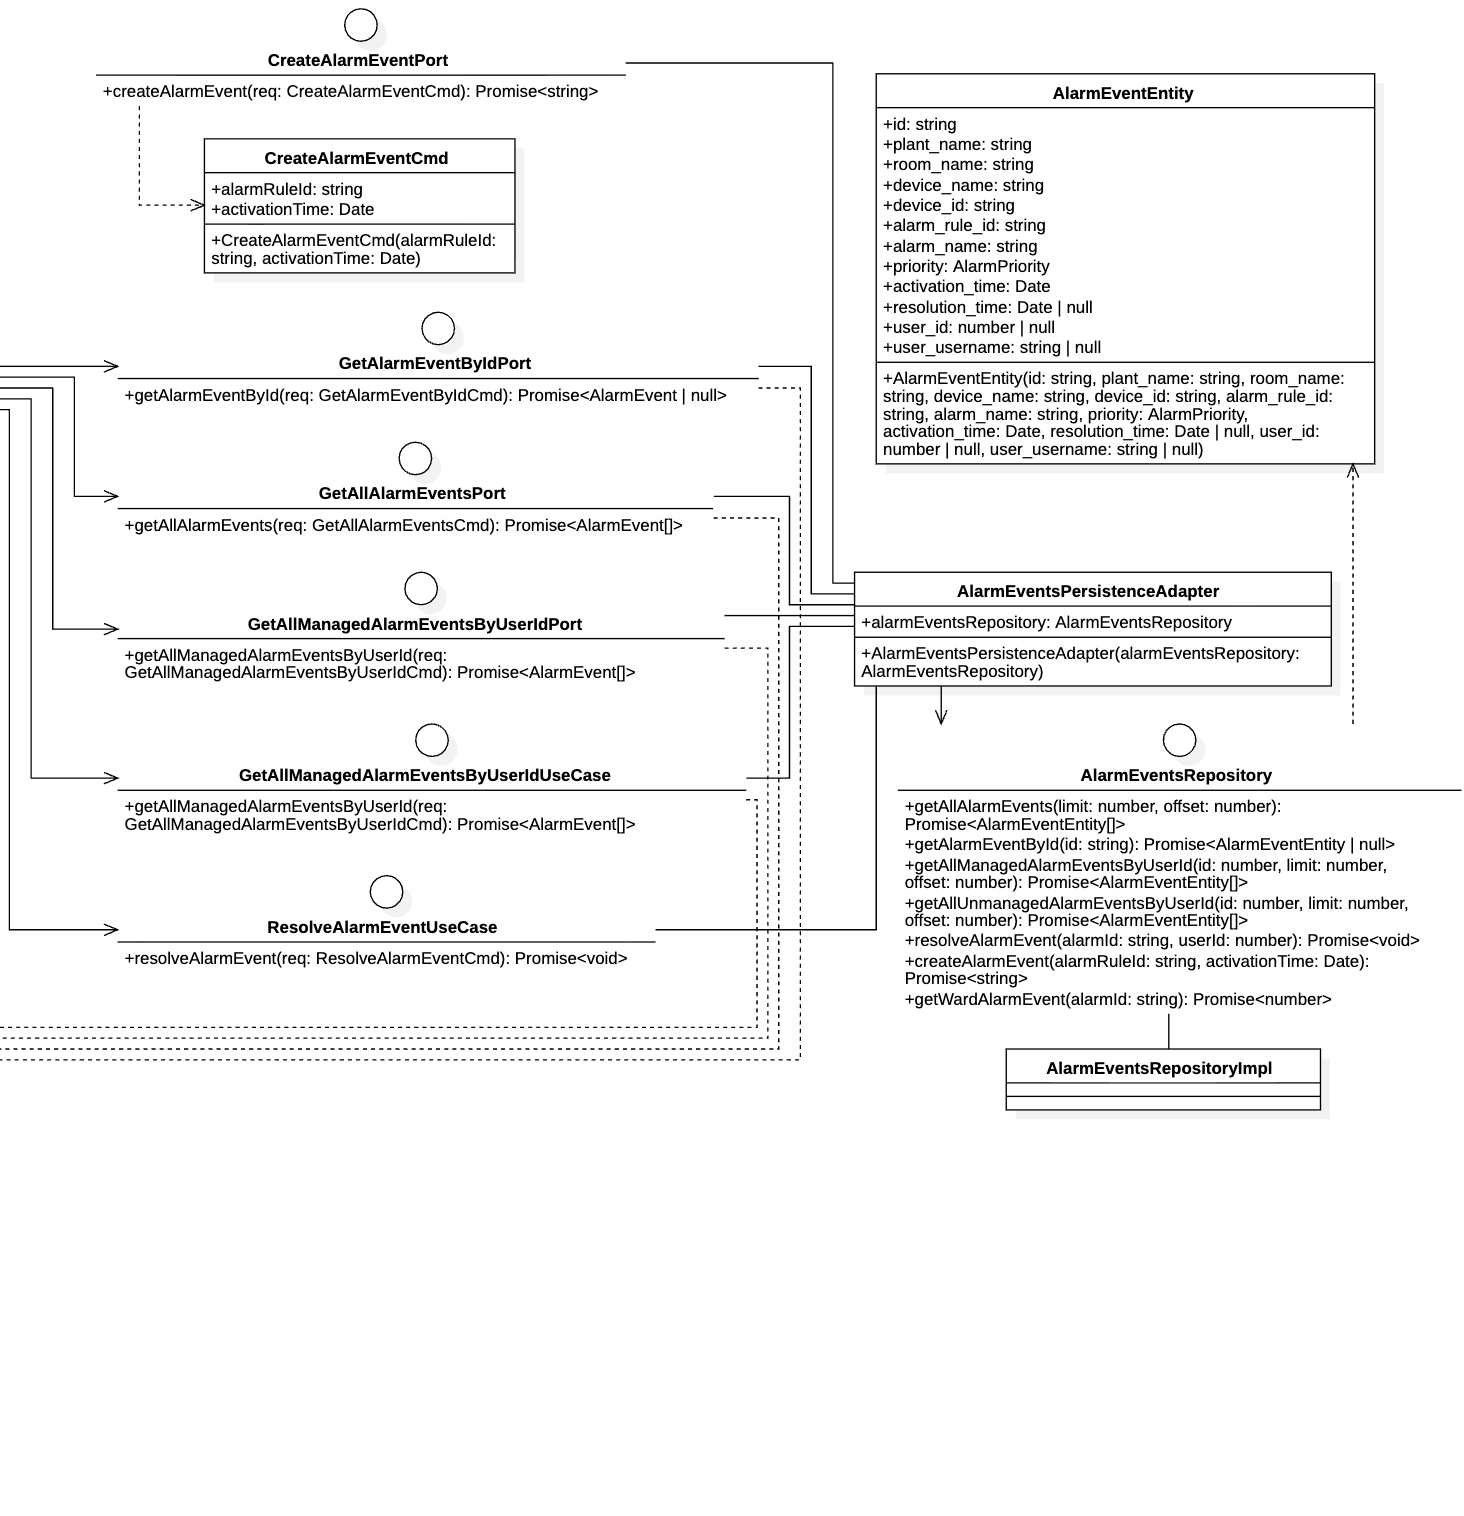
\includegraphics[width=0.95\textwidth]{img/AlarmUML2.png}
\end{center}
\end{frame}

\begin{frame}{Frontend: Architettura Model-View-ViewModel}
\begin{itemize}
  \item Problema:
  \begin{itemize}
    \item Logica di presentazione legata all'interfaccia utente;
    \item Ogni cambiamento della vista rischia di impattare la logica di business.
  \end{itemize}
  \item Soluzione: \textbf{Architettura MVVM} che separa le tre responsabilità:
\begin{itemize}
  \item \textbf{Model}: dati e logica di dominio, implementati come interfacce/tipi e come
        servizi (\texttt{@Injectable}).

  \item \textbf{View}: i template HTML del componente; passiva,
        si limita a realizzare le viste mostrando i dati via \textbf{property binding} e a
        notificare eventi via \textbf{event binding}.
  \item \textbf{ViewModel}: la classe del componente;
        fa da mediatore tra Model e View, esponendo i dati tramite
        \textbf{Observable} senza contenere logica di dominio.
\end{itemize}
\end{itemize}
\end{frame}

% \begin{frame}{Frontend: Architettura Model-View-ViewModel (2/2)}
% \begin{center}
%     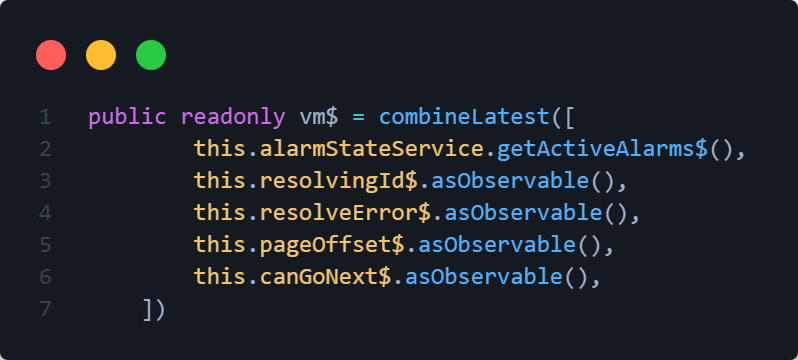
\includegraphics[width=0.8\textwidth]{img/viewmodel.png}
% \end{center}
% \end{frame}

\begin{frame}{UML Notification (Frontend)}
\begin{center}
  
\includegraphics[width=1.07\textwidth]{img/notification.pdf}
\end{center}
\end{frame}

\begin{frame}{Code snippets Notification (Frontend)}
  \begin{figure}
    \centering
    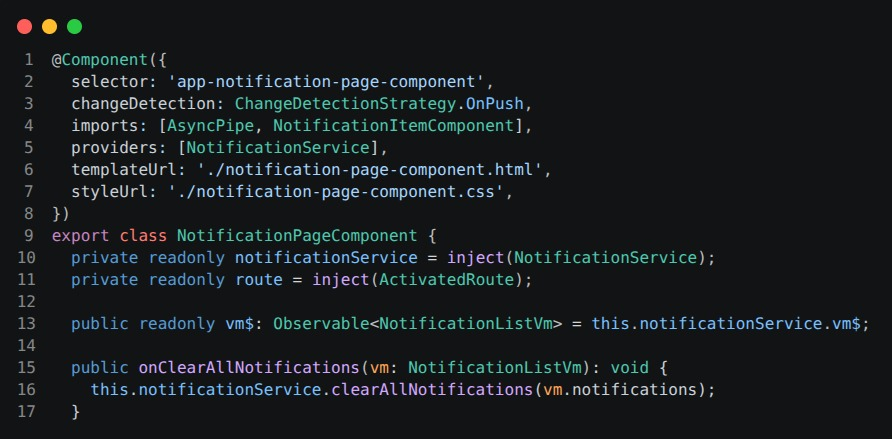
\includegraphics[width=0.6\textwidth]{img/vm_notification_component_snippet.png}
    \caption{notification-page-component.ts}
    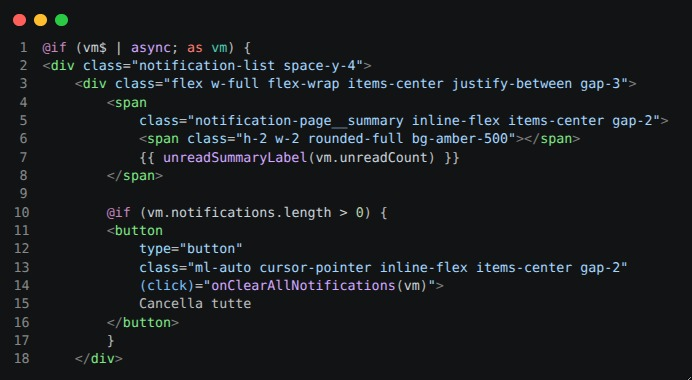
\includegraphics[width=0.6\textwidth]{img/vm_notification_template_snippet.png}
    \caption{notification-page-component}
  \end{figure}
    
  
  \end{frame}


\begin{frame}{Pattern - Dependency Injection (1/2)}
\begin{itemize}
  \item Problema:
        \begin{itemize}
          \item I moduli sono fortemente accoppiati tra di loro;
          \item Il codice risulta difficile da testare e da manutenere.
        \end{itemize}
  \item Soluzione: pattern \textbf{Dependency Injection}
          \begin{itemize}
            \item Le dipendenze vengono fornite tramite un \textit{injector};
            \item In \textit{TypeScript (NestJS/Angular)} il pattern è supportato nativamente tramite 
                  il decoratore \textit{@Injectable()} e il sistema \textit{providers}. 
          \end{itemize}
\end{itemize}
\end{frame}

\begin{frame}{Pattern - Dependency Injection (2/2)}
\begin{center}
    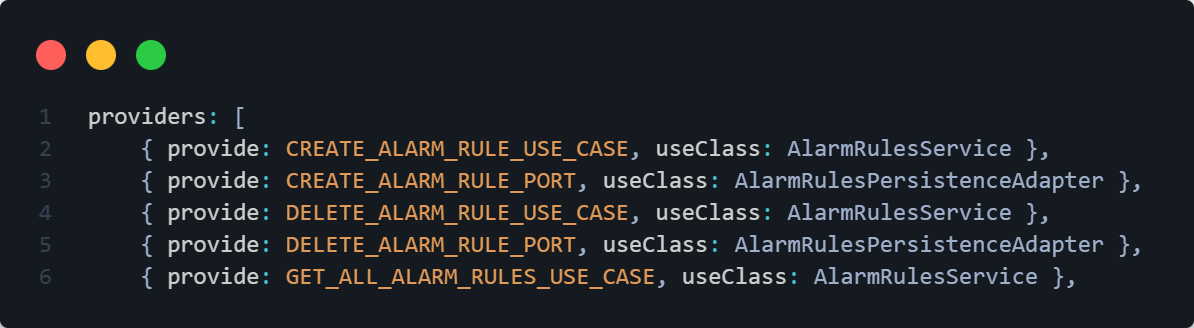
\includegraphics[width=0.8\textwidth]{img/providers.png}
    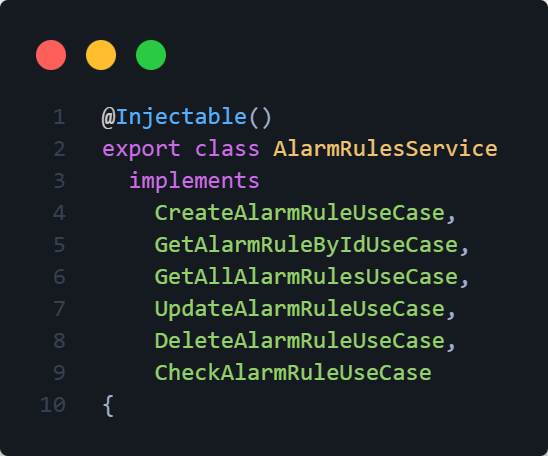
\includegraphics[width=0.4\textwidth]{img/injectable.png}
\end{center}
\end{frame}

\begin{frame}{Pattern - Observer (1/3)}
\begin{itemize}
    \item Problema:
    \begin{itemize}
      \item I componenti \textit{Angular} devono reagire a eventi asincroni (\textit{WebSocket}) 
      e sincronizzare lo stato \textit{UI}.
    \end{itemize}
    \item Soluzione: pattern \textbf{Observer}
    \begin{itemize}
      \item Implementato tramite \textit{RxJS}: le componenti si iscrivono 
      a \textit{Observable} senza conoscere la sorgente dei dati;
      \item Gli \textit{Observable} gestiscono in modo uniforme eventi asincroni e aggiornamenti di stato \textit{UI};
      \item La comunicazione tra componenti avviene tramite \textit{Subject} e \textit{BehaviorSubject} eliminando ogni accoppiamento diretto.
    \end{itemize}
\end{itemize}
\end{frame}

\begin{frame}{Pattern - Observer (2/3)}
\begin{center}
    UML
\end{center}
\end{frame}

\begin{frame}{Pattern - Observer (2/3)}
\begin{center}
  CODICE
    % 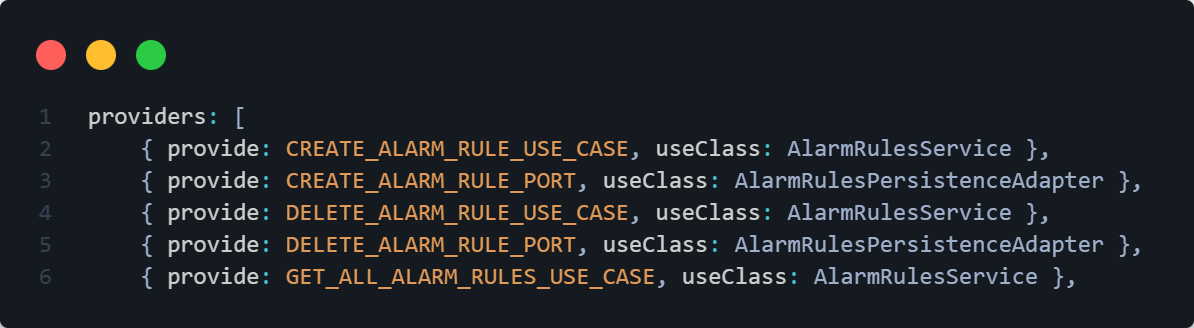
\includegraphics[width=0.8\textwidth]{img/providers.png}
\end{center}
\end{frame}

\begin{frame}{Pattern - Strategy (1/2)}
\begin{itemize}
  \item Problema: 
  \begin{itemize}
    \item Visualizzare un'insieme di \textit{analytics} relative agli impianti;
    \item Ogni \textit{analytics} ha un grafico specifico, basato su dati differenti (Es. consumo della luce, temperatura media del termostato, ecc.);
    \item Deve essere possibile modificare le \textit{analytics} se necessario.
  \end{itemize}
  \item Soluzione: \textbf{Pattern Strategy}
  \begin{itemize}
    \item È stata realizzata un'interfaccia \texttt{AnalyticsStrategy} che fornisce il metodo \texttt{execute}, che le \textit{strategies} implementano.
  \end{itemize}
\end{itemize}
\end{frame}

\begin{frame}{Pattern - Strategy (2/2)}
  \begin{center}
    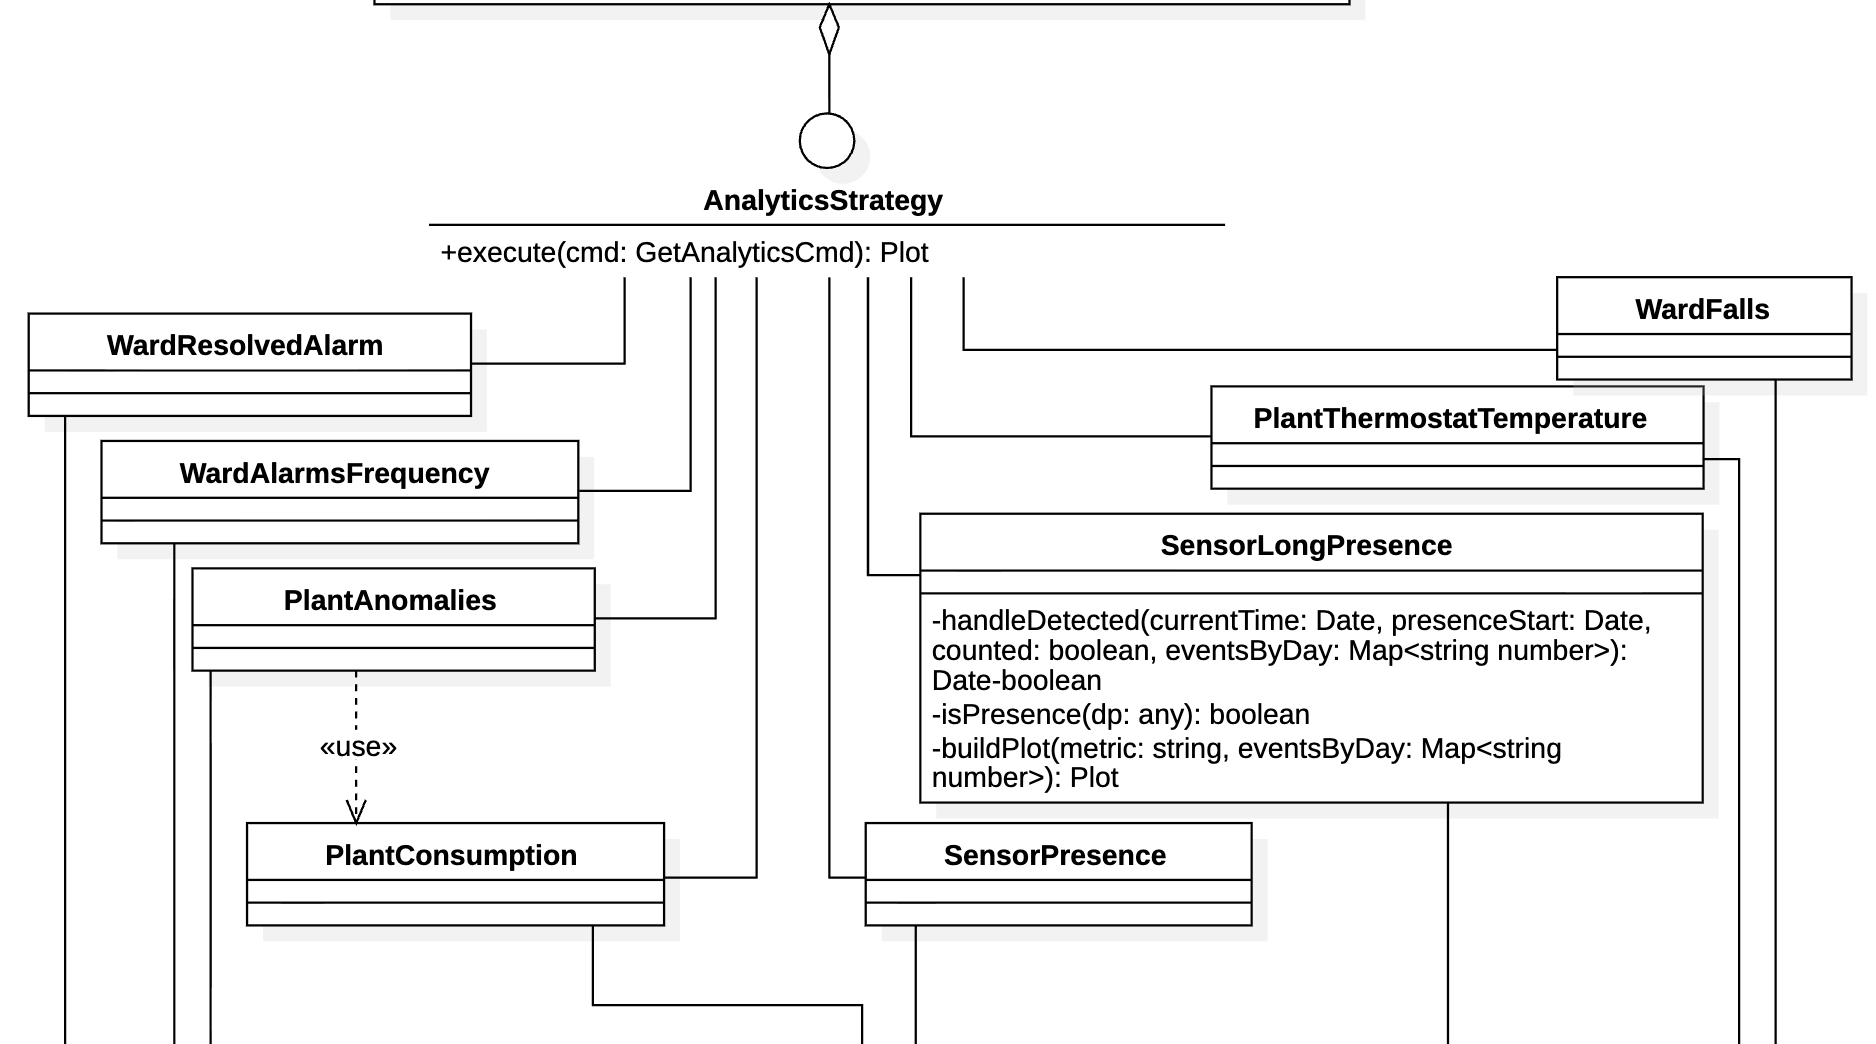
\includegraphics[width=1\textwidth]{img/strategy.png}
  \end{center}
\end{frame}

\end{document}